\chapter{Validação}

A seguir é descrita a estratégia de validação selecionada para este projeto, a mesma busca verificar a usabilidade e bom funcionamento do sistema, assim como aferir se o mesmo atende as expectativas dos usuários naquilo em que se propõe.

\section{Testes funcionais automatizados - API}
o motor deste projeto é a API que acessa os módulos auxiliares, através de um suíte de testes automatizados, foram testados os seguintes \textit{end-points} da API:

\begin{itemize}
    \item[a]) <IP>/api/: Sobre esta API;
    \item[b]) <IP>/api/auth: Devolve um token de autorização para acesso as áreas restritas da API;
    \item[c]) <IP>/api/devices: Retorna todos os dispositivos cadastrados;
    \item[d]) <IP>/api/users: Retorna todos os usuários cadastrados
\end{itemize}

A figura \ref{teste-api} mostra o resultado destes testes.

\begin{figure}[H]
\caption{\label{teste-api} Testes funcionais automatizados}
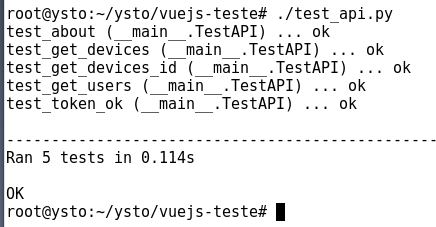
\includegraphics[scale=0.5]{img/test_api.png}
\legend{Fonte: Autor do projeto}
\end{figure}

\section{Embalagem e apresentação}
Por se tratar de uma proposta de produto, é importante que este esteja disposto de uma forma que facilite o seu manuseio. A figura \ref{prod-conceitual-01} mostra um conceito de embalagem para o módulo auxiliar.

\begin{figure}[H]
\caption{\label{prod-conceitual-01} Embalagem conceitual do módulo auxiliar}
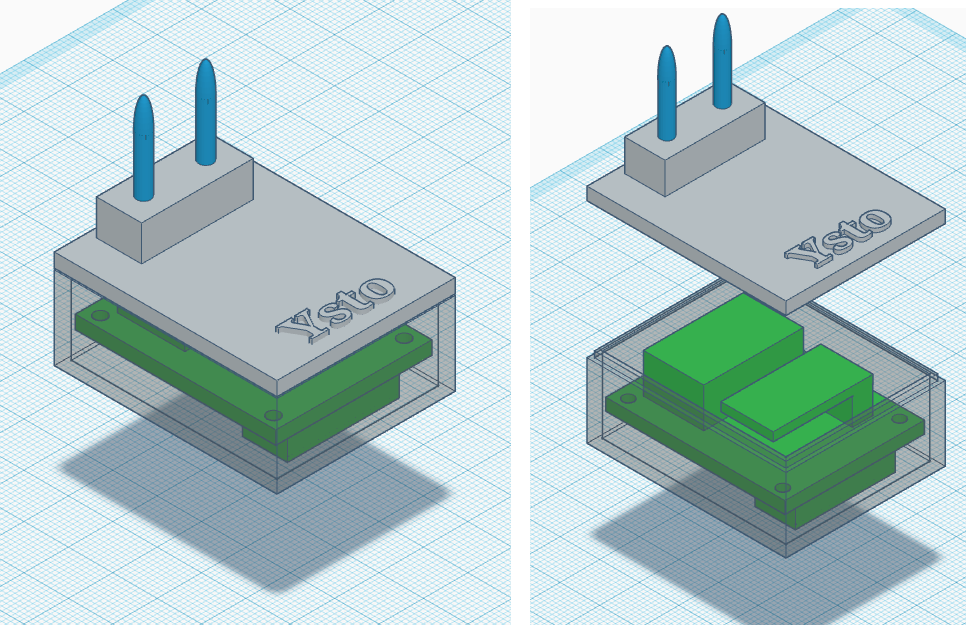
\includegraphics[scale=0.35]{img/12-prod-conceitual.png}
\legend{Fonte: Autor do projeto}
\end{figure}

Já a figura \ref{prod-rpi} usa um \textit{case} comercial para a RaspberryPI a central de controle.

\begin{figure}[H]
\caption{\label{prod-rpi} \textit{Case} comercial da central de controle}
\includegraphics[scale=0.15]{img/rpi.png}
\legend{Fonte: Autor do projeto}
\end{figure}


\section{Alcance de acionamento}
Os testes foram realizados com base em um terreno com 12 metros de frente por 30 metros de profundidade. Trata-se de um projeto que depende da qualidade do sinal da rede wifi, nestes ambientes sempre existe uma oscilação de sinal que deve ser desconsiderado para fins de testes práticos, em testes de laboratório isso poderia ser melhor explorado.

Para os testes do Módulo Auxiliar, o que impacta diretamente no desempenho de resposta é a qualidade da antena do módulo, em testes com variação de distância dentro do espaço descrito, ocorreram algumas falhas de acionamento quando nos limites do terreno. Um repetidor de sinal resolveria isso facilmente, não foi possível fazer esta verificação.

\section{Interface com usuário}
A idéia da interface com usuário é a de ser um painel de controle muito simples e de fácil manuseio, os conceitos foram repassados para uma família de 5 pessoas e para mais 2 pessoas de fora. Na época da explicação de como o projeto funciona, a interface com usuário não estava pronta e funcionando o que prejudica a analise do produto.

\section{Escopo e oportunidade}
Este projeto nasceu com uma proposta genéria de domótica residencial, não possuía nenhum cliente em potencial além das necessidades do próprio desenvolvedor. Este cenário mudou a partir do momento que outras pessoas passaram a tomar conhecimento do que este projeto se propunha a resolver e duas novas oportunidades surgiram.

\subsection{Sinalização para salas de espera}
Uma aplicação que não exigiria nenhuma adaptação da proposta atual seria a utilização do Ysto como um sinalizador de salas de consultórios médicos, onde é necessário avisar que um paciente chegou e está esperando. Este projeto pode ser usado para este fim uma vez que a recepcionista poderia administrar a central de controle e sempre que precisasse sinalizar para um médico em uma determinada sala, bastaria acionar o tópico correspondente a esta sala. Os tópicos poderiam ser formatados da seguinte forma, <NOME-DA-SALA>/saida. A carga a ser acionada pelo módulo auxiliar pode ser uma luminária comercial a gosto do decorador da clinica.

\subsection{Sinalização para praças de alimentação}
Da mesma forma uma praça de alimentação poderia utilizar de luminárias fixadas em suas mesas para fazer o controle e aviso de que o pedido está disponível, uma sugestão de tópico para este caso seria <MESA-CLIENTE>/saida.

\subsection{Situação atual}
Ambas possibilidades tem grande potencial e poderão se tornar uma proposta real, a idéia de utilizar como um sinalizador nasceu em uma conversa com a dona de uma clinica médica que viu neste projeto a possibilidade de uso em um curto espaço de tempo (em negociação).